%%%%%%%%%%%%%%%%%%%%%%%%%%%%%%%%%%%%%%%%%%
\section{Pressure Drop Across Packed Beds} \label{sec:modeling-pressure-drop}
%%%%%%%%%%%%%%%%%%%%%%%%%%%%%%%%%%%%%%%%%%
% Hill, Kock, \& Ladd\cite{Hill2001a}

% small Reynolds numbers

% simple cubic, face-centered cubic, random arrays

% drag force phi --> close-packed limits

% for small solid volume fraction, simulation similar to theory, therefore first inertial contribution to the drag force, when scaled with the Stokes drag force on a single sphere in open fluid, is proportional to the square of the Re #. Scaling persists --> close-packed limits.

% Inertial contribution to the drag force decreases with increasing solid volume fraction.

% Unsteady force is dominated by quasi-steady drag and added-mass forces.
%%%%%%%%%%%%%%%%%%%%%%%%%%%%%%%%%%%%%%%%%%
%\input{}
%%%%%%%%%%%%%%%%%%%%%%%%%%%%%%%%%%%%%%%%%%
\subsection{Kozeny-Carman Correlation for Pressure Drop}
P.C. Carman\cite{Carman1997}, using Kozeny's Equation as a starting point, derived a formula for the average velocity of a laminar flow through a randomly packed beds at the close-packed limit,

\begin{equation}\label{eq:K-C-velocity}
	U = \left(\frac{L}{L_e}\right)^2\frac{\epsilon^3}{k_0\mu S^2}\frac{\Delta p}{L}
\end{equation}

where $\mu$ is the viscosity, Carman called the tortuosity ($L_e/L$) the ratio of the actual path of a streamline through the pore space, $L_e$, to the length of packing, $L$. $S$ is the particle surface area per unit volume of the bed. For a bed of spheres this is $S = 6(1-\epsilon)/d_p$. The fluid void fraction, $\epsilon$ is obviously the complement to the packing fraction $\epsilon = 1 - \phi$ that we have used throughout this work. The constant, $k$, varies between materials and packings but for regular spheres is found experimentally to be $k\approx 5.0$. $\Delta p/L$ is the pressure drop per unit length of flow in the packed bed.

We rearrange Eq.~\ref{eq:K-C-velocity} as

\begin{equation}\label{eq:K-C-pressure}
	\frac{\Delta p}{L} = \frac{180 U \mu}{d_p^2} \frac{(1-\epsilon)^2}{\epsilon^3}
\end{equation}

The pressure gradient acting upon the fluid in the packed bed must be balanced by the drag force of all the particles in the bed. If we assume some average force, $\langle f \rangle$, as the ensemble average of the particle drag forces, we can write

\begin{equation}
	\frac{\Delta p}{L} = n \langle f \rangle
\end{equation}

where $n$ is the number density of particles in the bed. We relate the number density in terms of the packing fraction as

\begin{equation}
	n = \frac{6\phi}{\pi d_p^3} = \frac{6(1-\epsilon)}{\pi d_p^3}
\end{equation}

Thus the average drag per particle in this flow is

\begin{equation}\label{eq:average-drag}
	\langle f \rangle = \frac{\Delta p}{L}\frac{\pi d_p^3}{6(1-\epsilon)}
\end{equation}

We will non-dimensionalize the average drag force based on the classic Stokes force, drag force of a single particle in unbounded fluid,

\begin{equation}\label{eq:non-dim-drag}
	F = \frac{\langle f \rangle}{3\pi \mu d_p U}
\end{equation}

and when we plug in Eq.~\ref{eq:average-drag} to Eq.~\ref{eq:non-dim-drag} we have

\begin{equation}
	F_{kc} = \frac{\Delta p}{L}\frac{\pi d_p^3}{6(1-\epsilon)}\frac{1}{3\pi \mu d_p U}
\end{equation}

which, with the substitution of the Kozeny-Carman pressure (Eq.~\ref{eq:K-C-pressure}), becomes

\begin{equation}
	F_{kc} = \frac{180 U \mu}{d_p^2} \frac{(1-\epsilon)^2}{\epsilon^3}\frac{\pi d_p^3}{6(1-\epsilon)}\frac{1}{3\pi \mu d_p U}
\end{equation}

or simply

\begin{equation}\label{eq:K-C-non-dim}
	F_{kc} = 10\, \frac{1-\epsilon}{\epsilon^3}
\end{equation}

Carman points out\cite{Carman1956} the limitations of the Kozeny-Carman equation. Built into the equation is the assumption that the range of pore size and shape is fairly isotropic and similarly the tortuosity through the packed bed is relatively uniform. In the form we have used with Eq.~\ref{eq:K-C-non-dim}, we have also assumed spherical particles in random packing near the close-packed limit ($\phi \rightarrow 0.64$) with laminar flow at low Reynolds numbers. Carman provided modifications to cases of extremely high porosity and non-spherical, non-regular packings in his book from 1956.\cite{Carman1956}

\subsection{Ergun Correlation for Pressure Drop}

Another correlation that is perhaps more commonly used in general is the Ergun equation.\cite{ergun1952fluid} Ergun's correlation is an empirical fit to a vast amount of experimental data. His pressure drop per length is 

\begin{equation}\label{eq:ergun-pressure}
	\frac{\Delta p}{L} = \frac{150 U \mu}{d_p^2} \frac{(1-\epsilon)^2}{\epsilon^3} + \frac{1.75 \rho U^2}{d_p}\frac{1-\epsilon}{\epsilon^3}
\end{equation}

We non-dimensionalize the Ergun equation of Eq.~\ref{eq:ergun-pressure} in the same form as Eq.~\ref{eq:K-C-non-dim} to find

\begin{equation}\label{eq:ergun-non-dim}
	F_e = 8.33 \, \frac{1-\epsilon}{\epsilon^3} + 0.18 \, \frac{\Re}{\epsilon^3}
\end{equation}

where we see the Reynolds number dependence in the second term on the right side of Eq.~\ref{eq:ergun-non-dim}. Comparing this to the non-dimensionalized drag force of the Kozeny-Carman relation (Eq.~\ref{eq:K-C-non-dim}), we see that the first term on the right hand side is essentially the same but Ergun's equation underpredicts Stokes flow by roughly 20\% (8.33 to 10.0). This is understandable as Ergun's equation was meant to fit a wide range of flow (finite-to-large $\Re$), including turbulent flow, whereas the Kozeny-Carman was meant specifically to apply to Stokes flow-type laminar packed beds.

\subsection{Koch-Hill-Lad Correlation for Pressure Drop}
Koch, Hill, \& Ladd studied packed bed flow with high-precision lattice-Boltzmann simulations to develop correlations for drag in a packed bed over a wide range of packing fractions and Reynolds numbers.\cite{Koch2001,Hill2001a,Hill2001} They studied ordered arrays of spheres at various flow angles with dilute arrays (interstitial Reynolds number greater than particle Reynolds number), up to dense ordered arrays, and random arrays.

They consider the drag force as a sum of viscous and inertial stresses. Based on scaling arguments, the viscous and inertial contributions to $F$ are expected to be independent of $\Re$ and linearly proportional to $\Re$, respectively (in much the same form as Ergun's empirical fit of Eq.~\ref{eq:ergun-non-dim}). Thus their numerical results were fit to the form

\begin{equation}
	F = F_0(\phi) + F_3(\phi)\Re
\end{equation}

where 

\begin{equation}
F_0 = \begin{cases}
	\frac{1+3(\phi/2)^{1/2} + (135/64)\phi\ln\phi + 16.14\phi}{1 + 0.681\phi - 8.48 \phi^2 + 8.16\phi^3} & \text{if $\phi < 0.4$}\\
	10.0\,\frac{\phi}{(1-\phi)^3} & \text{if $\phi > 0.4$} 
	\end{cases}
\end{equation}

and

\begin{equation}
	F_3 = 0.0673 + 0.212\phi + 0.0232 \frac{1}{(1-\phi)^5}
\end{equation}

Koch, Hill, \& Ladd\cite{Hill2001} compare their results with data from experiments. They found that at smaller Reynolds number and larger solid volume fractions, the rate of increase of drag force increases with the Reynolds number in much the same way predicted by Ergun’s equation. However, at solid volume fractions smaller than those that can be achieved in physical experiments, at the largest Reynolds numbers, the rate of drag force increase is significantly smaller than the value predicted by Ergun's equation.

For Stokes-flow (and near-Stokes-flow), the drag force computed from their lattice-Boltzmann simulations were indistinguishable from experimental data over all ranges of packing fractions achievable in controlled experiments. The correlation fit to their data for small Reynolds number and large packing fraction is simply the Kozeny-Carman relationship -- which was itself generated with coefficients matching experimental data so it is no surprise their correlation fits that phase space of $\phi-\Re$.

\subsection{Correlation Comparisons}
We have given three correlations relating a non-dimensional drag force to packing fraction and Reynolds number. The first, the Kozeny-Carman equation, is applicable at small Reynolds number and broad range of packing fraction. The second, the Ergun equation, is applicable at a broad range of Reynolds number but is most accurate at higher packing fractions and also under-predicts drag at low Reynolds numbers. Finally, the third correlation by Koch, Hill, \& Ladd (KHL), extended the drag correlations over a much more broad packing fraction and Reynolds numbers than is possible with physical experiments. 

Here we simply provide a graphical comparison of the relationships that demonstrates when the classic correlations of Kozeny-Carman and Ergun match the correlation of KHL and when they diverge.
\begin{figure}[!ht]
	\centering
	\begin{subfigure}[b]{0.45\textwidth}
		\centering
		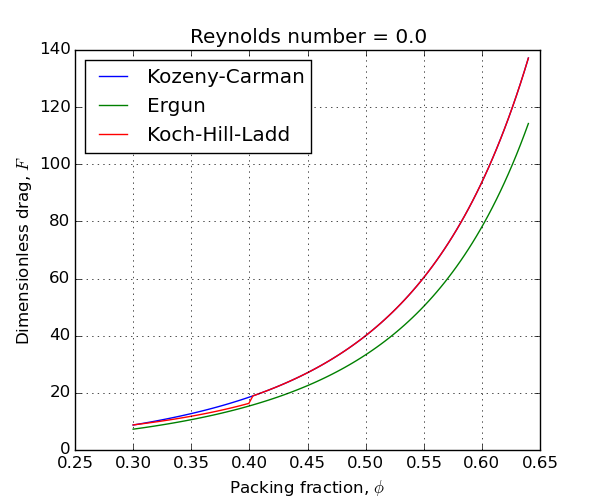
\includegraphics[width=\textwidth]{chapters/figures/pressure-drop-correlations/Re0.png}
	\end{subfigure}
	\begin{subfigure}[b]{0.45\textwidth}
		\centering
		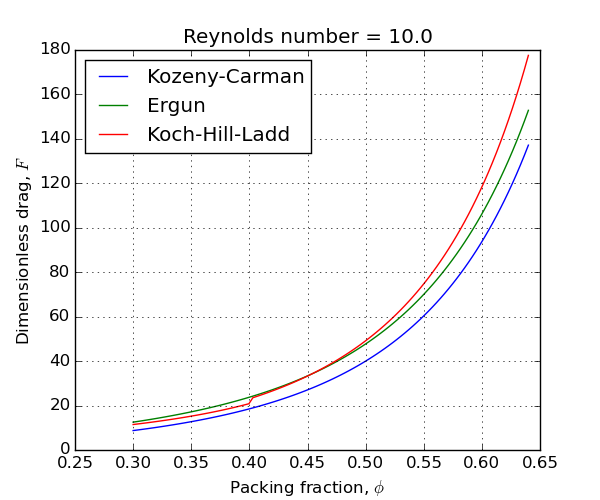
\includegraphics[width=\textwidth]{chapters/figures/pressure-drop-correlations/Re10.png}
	\end{subfigure}
	
	\begin{subfigure}[b]{0.45\textwidth}
		\centering
		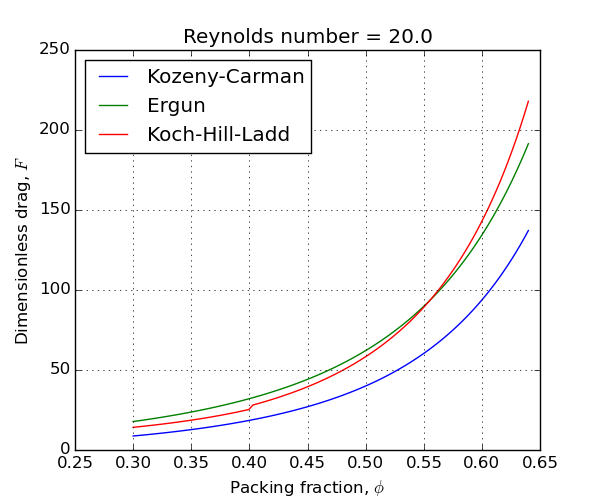
\includegraphics[width=\textwidth]{chapters/figures/pressure-drop-correlations/Re20.png}
	\end{subfigure}
	\begin{subfigure}[b]{0.45\textwidth}
		\centering
		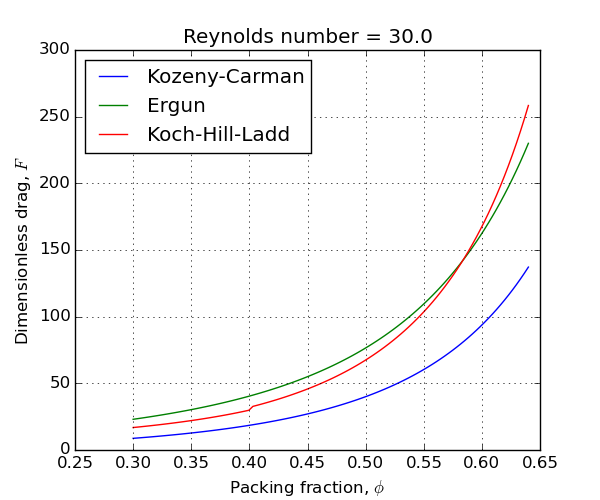
\includegraphics[width=\textwidth]{chapters/figures/pressure-drop-correlations/Re30.png}
	\end{subfigure}

	\begin{subfigure}[b]{0.45\textwidth}
		\centering
		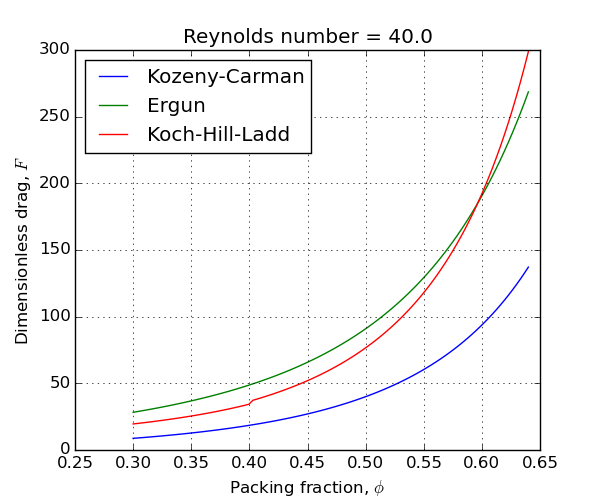
\includegraphics[width=\textwidth]{chapters/figures/pressure-drop-correlations/Re40.png}
	\end{subfigure}
	\begin{subfigure}[b]{0.45\textwidth}
		\centering
		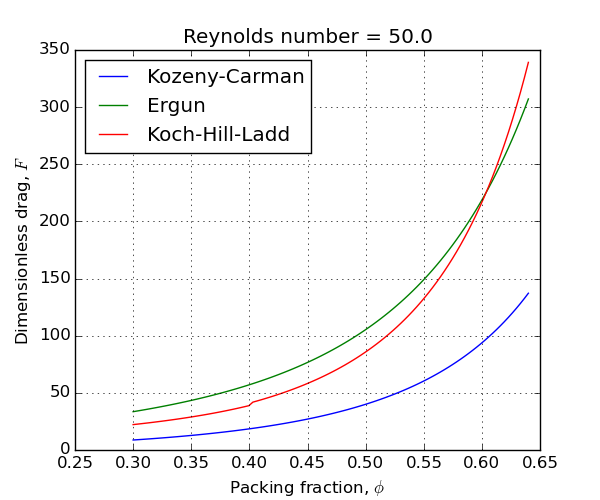
\includegraphics[width=\textwidth]{chapters/figures/pressure-drop-correlations/Re50.png}
	\end{subfigure}
	\caption{Comparison of pressure drop correlations over a range of packing fractions and Reynolds numbers.}
\label{fig:p-drop-correlations}
\end{figure}

Later, in \cref{sec:modeling-cfd-dem}, we will return to these correlations as we discuss the computational groundwork of the CFD-DEM coupling routine.



\FloatBarrier